\documentclass[a4paper,12pt]{article}

\usepackage[utf8]{inputenc}
\usepackage[T1]{fontenc}
\usepackage{textcomp}
\usepackage[english]{babel}
\usepackage{amsmath, amssymb}
\usepackage[top=1in,bottom=1in,left=1in,right=1in]{geometry}
%\usepackage[margin=1in]{geometry}
\usepackage[onehalfspacing]{setspace}
%\usepackage[doublespacing]{setspace}
\usepackage[none]{hyphenat}
\usepackage{enumitem}

%figure support
\usepackage{import}
\usepackage{xifthen}
\pdfminorversion=7
\usepackage{pdfpages}
\usepackage{transparent}
\newcommand{\incfig}[1]{%
	\def\svgwidth{\columnwidth}
	\import{./figures/}{#1.pdf_tex}
}
\graphicspath{ {./figures/} }
\pdfsuppresswarningpagegroup=1

\begin{document}
	\title{CIS4362.01 Homework 2 Due: 10/13/19}
	\author{Brandon Thompson 5517}
	\maketitle

	\begin{enumerate}
		\item Let G:K $\to \left\{ 0,1 \right\}^{n} $ be a secure PRG. Define
			$G'\left( k_1,k_2 \right) = G\left( k_1 \right) \oplus G\left( k_2 \right) $.\\
			Consider the following statistical test $A$ on $\left\{ 0,1 \right\}^{n} $,\\
			$A\left( x \right) $ outputs $LSB\left( x \right) $, the least significant bit if $x$.\\
			What is $Adv_{PRG}\left[ A, G' \right] $?\\
			You may assume that $LSB\left( G\left( k \right)  \right) $ is 0 for exactly
			half the seeds $k \in K$.\\
			\\
			Advantage Formula:\\$Adv_{PRG}\left[ A,G \right] = \left| Pr_{k \leftarrow K}\left[ A\left( G\left( k \right)  \right) = 1 \right] - Pr_{r \leftarrow \left\{ 0,1 \right\}^{n}} \left[ A\left( r \right) = 1 \right]  \right| \in \left[ 0,1 \right] $\\
			\begin{align*}
				Pr\left[A\left( G\left( k_1 \right)  \right) = 1 \right] & = \frac{1}{2}\\
				\\
				Pr\left[A\left( G\left( k_2 \right)  \right) = 1 \right] & = \frac{1}{2}\\
				\\
				Pr\left[ A\left( G\left( k_1 \right) \oplus G\left( k_2 \right) \right) =1 \right]  & = \frac{1}{2}\\
				\\
				Pr\left[ A\left( r \right) = 1 \right]  & = \frac{1}{2}\\
				\\
				{\bf Adv_{PRG} = \left|\frac{1}{2}-\frac{1}{2} \right|  & = 0}
			\end{align*}
			\newpage
		\item Recall that the Luby-Rackoff theorem discussed in \emph{The Data Encryption Standard lecture}
			states that applying a \textbf{three} round Feistal network to a secure PRF gives a
			secure block cipher. Let's see what goes wrong if we only use a \textbf{two} round
			Feistal.\\
			Let F:K $\times \left\{ 0,1 \right\}^{32} \to \left\{ 0,1 \right\}^{32} $ be a secure PRF.\\
			Recall that a 2-round Feistal defins the following PRP\\
			$F_2: K^2\times \left\{ 0,1 \right\}^{64} \to \left\{ 0,1 \right\}^{64} } $ \\
			%image of Feistal network
			\\
			Here $R_0$ is the right 32 bits of the 64-bit input and $L_0$ i the left 32-bits.\\
			\\
			One of the following lines is the output of this PRP $F_2$ using a random key, while
			the other three are the output of a truly random permutation
			$f:\left\{ 0,1 \right\}^{64} \to \left\{ 0,1 \right\}^{64} $.
			All 64-bit outputs are encoded as 16 hex characters.\\
			\\
			Can you say which is the output of the PRP\? Note that since you are able to distinguish
			the output of $F_2$ from random, $F_2$ is not a secure block cipher, which is what we
			wanted to show.\\
			\textbf{Hint:} First argue that there is detectable pattered in the xor of
			$F_2$\\
			\\
			{\bf On input $0^{64}$ the output is ''e86d2de2 e1387ae9''. On input $1^{32}0^{32}$ the
			output is ''1792d21d b645c008''.}
		\item Nonce-based encryption has been implemented in HTTPS and IPSec design. Please explain
			how nonce has been implemented in these two protocols.
			\begin{description}
				\item[HTTPS:] Nonce is used to validate credentials of clients and servers,
					calculate MD5 hashes for passwords. Because the nonce is different
					every time it makes replay attacks virtually impossible.
				\item[IPSec:] Nonce is used to allow repeated use of private Diffie Hellman
					parameters
			\end{description}
			\pagebreak
		\item Let $m$ be a message consisting of $\ell$ AES blocks (say $\ell=100$ ). Alice encrypts
			$m$ using CBC mode and transmits the resulting ciphertext to Bob. Due to a network
			error, ciphertext block number $\frac{\ell}{2}$ is corrupted during transmission.
			All other ciphertext blocks are transmitted and received correctly. Once Bob decrypts
			the received ciphertext, how many plaintext blocks will be corrupted?\\
			% image of CBC mode
			\begin{figure}[h!]
				\centering
				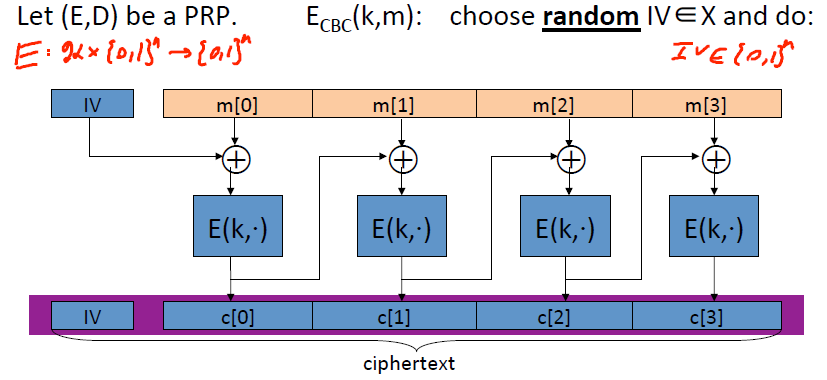
\includegraphics[width=0.8\textwidth]{cbc_mode}
				\caption{CBC Mode}
				\label{fig:cbc_mode}
			\end{figure}
			\\Because the previous ciphertext is used in the calculating the next ciphertext,
			if one is corrupted in transmission then it is used in decrypting two ciphertexts.
			\pagebreak
		\item Let $m$ be a message consisting of $\ell$ AES blocks (say $\ell=100$ ). Alice encrypts
                        $m$ using randomized counter mode and transmits the resulting ciphertext to Bob.
			Due to a network error, ciphertext block number $\frac{\ell}{2}$ is corrupted during
			transmission. All other ciphertext blocks are transmitted and recieved correctly.
			Once Bob decrypts the received ciphertext, how many plaintext blocks will be corrupted?
			%image of rand ctr. mode
			\begin{figure}[h!]
				\centering
				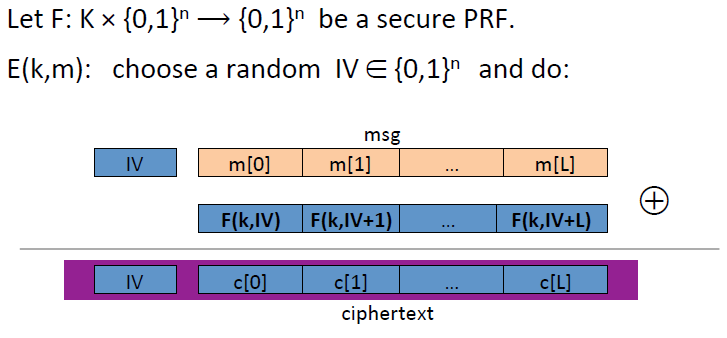
\includegraphics[width=0.8\textwidth]{rand_ctr_mode}
				\caption{Randomized Counter Mode}
				\label{fig:rand_ctr_mode}
			\end{figure}
			\\
			Because no previous ciphertexts are used in encrypting, if one is corrupted during
			transmission it will only effect the same message block.\\\\
		\item Nonce-based CBC. Recall that we said that if one wants to use CBC encryption with a
			non-random unique nonce then the nonce must first be encrypted with an \textbf{independent}
			PRP key and the result then used as the CBC IV.\\
			\\
			Let's see what goes wrong if one encrypts the nonce with the \textbf{same} PRP key as
			the key used for CBC encryption.\\
			\\
			Let $F:K\times \left\{ 0,1 \right\}^{\ell} \to \left\{ 0,1 \right\}^{\ell}$ be a secure
			PRP with, say $\ell=128$. Let $n$ be a nonce and suppose one encrypts a message $m$
			by first computing  $IV=F\left( k,n \right)$ and then using this IV in CBC encryption
			using $F\left( k,\cdot \right)$. Note that the same key $k$ is used for computing
			the IV and for CBC encryption. We show that the resulting system is not nonce-based
			CPA secure.\\
			\\
			The attacker begins by asking for the encryption of the two block message
			$m=\left( 0^{\ell},0^{\ell} \right)$ with nonce $n=0^{\ell}$. It receives back a two
			block ciphertext $\left( c_0,c_1 \right) $. Observe that by definition of CBC we know
			that $c_1=F\left( k,c_0 \right) $.\\
			\\
			Next, the attacker asks for the encryption of the one block message $m_1=c_0 \oplus c_1$
			with nonce $n=c_0$. It receives back a once block ciphertext $c_0'$.\\
			\\
			What relation holds between $c_0,c_1,c_0'$? Note that this relation lets the adversary
			win the nonce-based CPA game with advantage 1.\\
			\begin{figure}[h!]
				\centering
				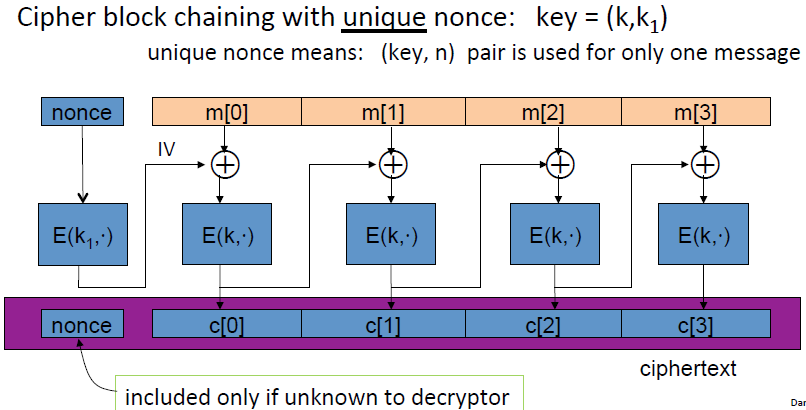
\includegraphics[width=0.8\textwidth]{nonce_cbc}
				\caption{Nonce-based CBC}
				\label{fig:nonce_cbc}
			\end{figure}
			\begin{align*}
				\text{Nonce} &= 0^{128}\\
				m_0 &= \left( 0^{128},0^{128} \right) \\
				F\left( k,\text{nonce} \right) &= IV\\
				F\left( m_0 \oplus IV\right) &= \left( c_0,c_1 \right) \\
				c_1 &= F\left( k,c_0 \right) \\
				\text{Nonce} &= c_0\\
				m_1 &= \left( c_0 \oplus c_1 \right) \\
				F\left( k,\text{nonce} \right) &= c_1 \text{\em\ \ \ \ See line 5}\\
				F\left( k,c_1 \oplus \left( c_0 \oplus c_1 \right)  \right) &= c_0'
			\end{align*}
			{\bf The association between $c_0,c_1,c_0'$ is that $c_0=c_0'$.}
			\pagebreak
		\item What is the corresponding ciphertext for the below message if CBC with random IV is
			used for encryption.\\
			\textbf{Note:}
			\begin{enumerate}[label=\roman*.]
				\item {\em Suppose that the underlying block cipher is AES.}
				\item {\em The $E\left( k,\cdot \right)$ function shifts the input, 1 bit
					to the left.}
				\item {\em Suppose each item in the array cell is just one byte.}
				\item {\em  Make sure that you append the padding block before encrypting.}
			\end{enumerate}
			%image for array
			\begin{figure}[h!]
				\centering
				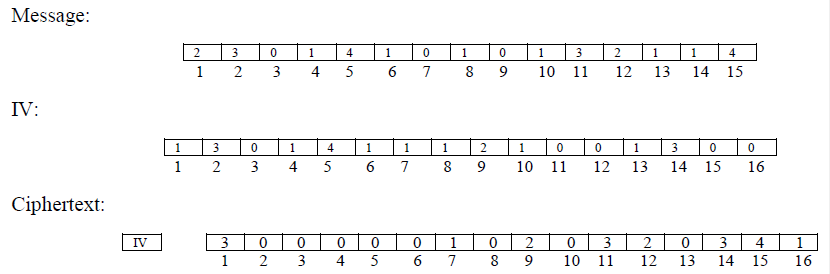
\includegraphics[width=0.8\textwidth]{question7}
				\caption{Answer to question 7}
				\label{fig:question7}
			\end{figure}
		\item Given the following messages with different length for encryption through CBC mode,
			\emph{Identify the padding block size and content for each message. Suppose the
			underlying block cipher is AES.} In addition, suppose each character is one byte.
			%image for message padding
			\begin{figure}[h!]
				\centering
				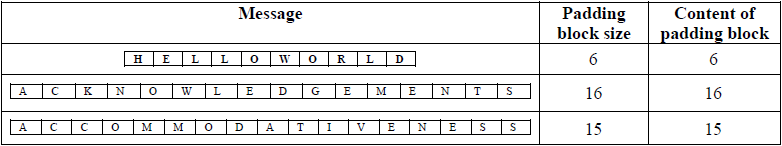
\includegraphics[width=0.8\textwidth]{question8}
				\caption{Answer to question 8}
				\label{fig:question8}
			\end{figure}

		\end{enumerate}
\end{document}
